\documentclass[fleqn]{MJDArticle}
%%%%%%%%%%%%%%%%%%%%%%%%%%%%%%%%%%%%%%%%%%%%%%%%%%%%%%%%%%%%%%%%%%%%%%%
\begin{document}
\titleAT[Abstract Outline]{Matthew Denny}

\section{Gender in Organizations}

\begin{enumerate}
	\item Gender bias in organizations is well documented in terms of pay, prestige, position, and social interaction. 
	\item Gender equity is normatively important.
	\item Scholars have sought to understand the roots, extent, and nature of gender bias, but have not had access to primary source data. This has traditionally been observational, ethnographic and self reports, which can be biased. Limited in scope. 
	\item With the increasing use of electronic communication, and the rise of e-government/ transparency, we are now able to use government email to study gender bias using primary source data.
	\item This also makes our analyses replicable. 
	\item Therefore, we choose to explore the relationship between gender and communication patterns in government organizations. 
	% gender in govt organizations has been studies before pulbic vs. private. 
	\item To do this, we collect and analyze large scale email data from a sample of 17 local governments.  
	\item What do we look for, how do we do it,  what do we find -- at a high level. 
\end{enumerate}

\section{Data}

\begin{enumerate}
	\item North Carolina has robust public records laws which let us collect data.
	% \item We did this as part of a transparency-by-conformity field experiment. Make sure to spell out what we do.
	\item 22 complied with our request but only 17 counties did so in a way that  was  useful to our research, allowing us to compare across organizations.
	\item Provide some descriptive statistics of the data.
	\begin{figure}[H]
		\centering
	\caption{\label{fig:nc map} North Carolina county map.}	
	\centering
	
\includegraphics[width = 0.48\textwidth]{images/County_Map.pdf}
	\end{figure}
	
	\begin{table}[H]
	\centering
		\begin{tabular}{lrrrrr}
		  \hline
		  % add an extra line
		  & \multicolumn{2}{c}{\textbf{Manager Gender}} & \multicolumn{2}{c}{\textbf{Email Sender}}\\
		 \textbf{County} & \textbf{Male} & \textbf{Female} & \textbf{Manager} &\textbf{All} \\
		  \hline
		Alexander & 12 & 9 & 907 & 11,924  \\
		Caldwell & 12 & 8 & 121 &    \\
		Chowan & 12 & 11 & 2,027 & 11,737  \\
		Columbus & 14 & 10 & 920 & 12,707  \\
		Dare & 15 & 12 & 2,247 &   \\
		Duplin & 13 & 14 & 1,914 &   \\
		Hoke & 13 & 11 & 1,106 & 5,565  \\
		Jackson & 18 & 6 & 1,499 &   \\
		Lenoir & 15 & 5 & 560 & 10,499 \\
		Lincoln & 15 & 7 & 573 & 8,727  \\
		McDowell & 12 & 5 & 326 & 3,494  \\
		Montgomery & 8 & 10 & 680 & 2,465  \\
		Nash & 11 & 8 & 1,147 & 9,133 \\
		Person & 12 & 9 & 1,491 & 14023  \\
		Transylvania & 16 & 4 & 1,857 & 14,088 \\
		Vance & 10 & 8 & 185 & 4,349  \\
		Wilkes & 15 & 2 & 303 & 8,443  \\
		   \hline
		   \textbf{Totals:} & 362 & 139 & 17,863 & 117,154  \\
		   \hline
		\end{tabular}
		\caption{\label{tab:county aggregate stats}Participating county email statistics. \textbf{Mgrs.} is the total number of department managers in a county, \textbf{Female} is the number of female managers in that county, \textbf{Internal} is the number of emails sent between managers in a county, and \textbf{Total} is the total number of emails sent and received by department managers in each county in our sample. Note that in this study, we only make use of the internal email data. Some email \textbf{Total}'s are omitted due to challenges in determining which emails (not sent by managers) were valid in these counties.}
	\end{table}

	\item These counties are a representative sample and we have tons of data so lets start analyzing it.

\end{enumerate}


\section{Descriptive Analysis}
\begin{enumerate}
	
	\item We want to see if there is a relationship between sender gender and recipient gender.
	\item If we want to know about gendered patterns of communication in organizations, we should start by looking at aggregate statistics by gender:
	
	
	\begin{table}[H]
	\centering
		\begin{tabular}{m{2in}rrr}
		\toprule
	& \textbf{Male} & \textbf{Female}  \\
		 \midrule
		 Proportion of Managers in Sample & 61.6\%& 38.4\% \\
		 \midrule
		 Average \# Emails Sent & 48.3 & 51 \\
		 Average \# Recipients Per Email Sent & 1.45 & 1.43 \\
		 \midrule
		 Average \# Emails Received & 70.8 & 71.6 \\
		\bottomrule
		\end{tabular}
		\caption{\label{tab:email agg stats}Manager email statistics by gender.}
	\end{table}
	
	
	\item To test for independence, we construct a contingency table of email sender gender against email recipient gender. We then perform a $\chi^2$ test for independence between the rows and columns.
	
	% make this a contingency table and do a chi squared test
	\begin{table}[H]
	\centering
		\begin{tabular}{lrrrr}
		\toprule
	& \textbf{Male Recipient} & \textbf{Female Recipient} & \textbf{Total}  \\
		 \midrule
		 \textbf{Male Sender} & 7,299 & 6,286 & 13,585 \\
		 \textbf{Female Sender} & 5,325 & 3,510 & 8,835 \\
		 \textbf{Total} & 12,624 & 9,796 & 22,420\\
		\bottomrule
		\end{tabular}
		\caption{\label{tab:email agg stats}Manager gender contingency table.}
	\end{table}
	
	\item The test statistic is $\chi^2 = 92.9$ with a p-value $< 0.00001$, indicating that the gender of an email sender and its recipients is not independent. 
	
	\item We have replicated previous research, we do see gender bias, we could stop here but because we have more information we are going to dig deeper.

	\item One place the literature tells us to look for gender bias is in the roles/positions in the organization.
	
	\item \textbf{Add in a gender vs. position table here}
	
	\begin{figure}[H]
	\centering
	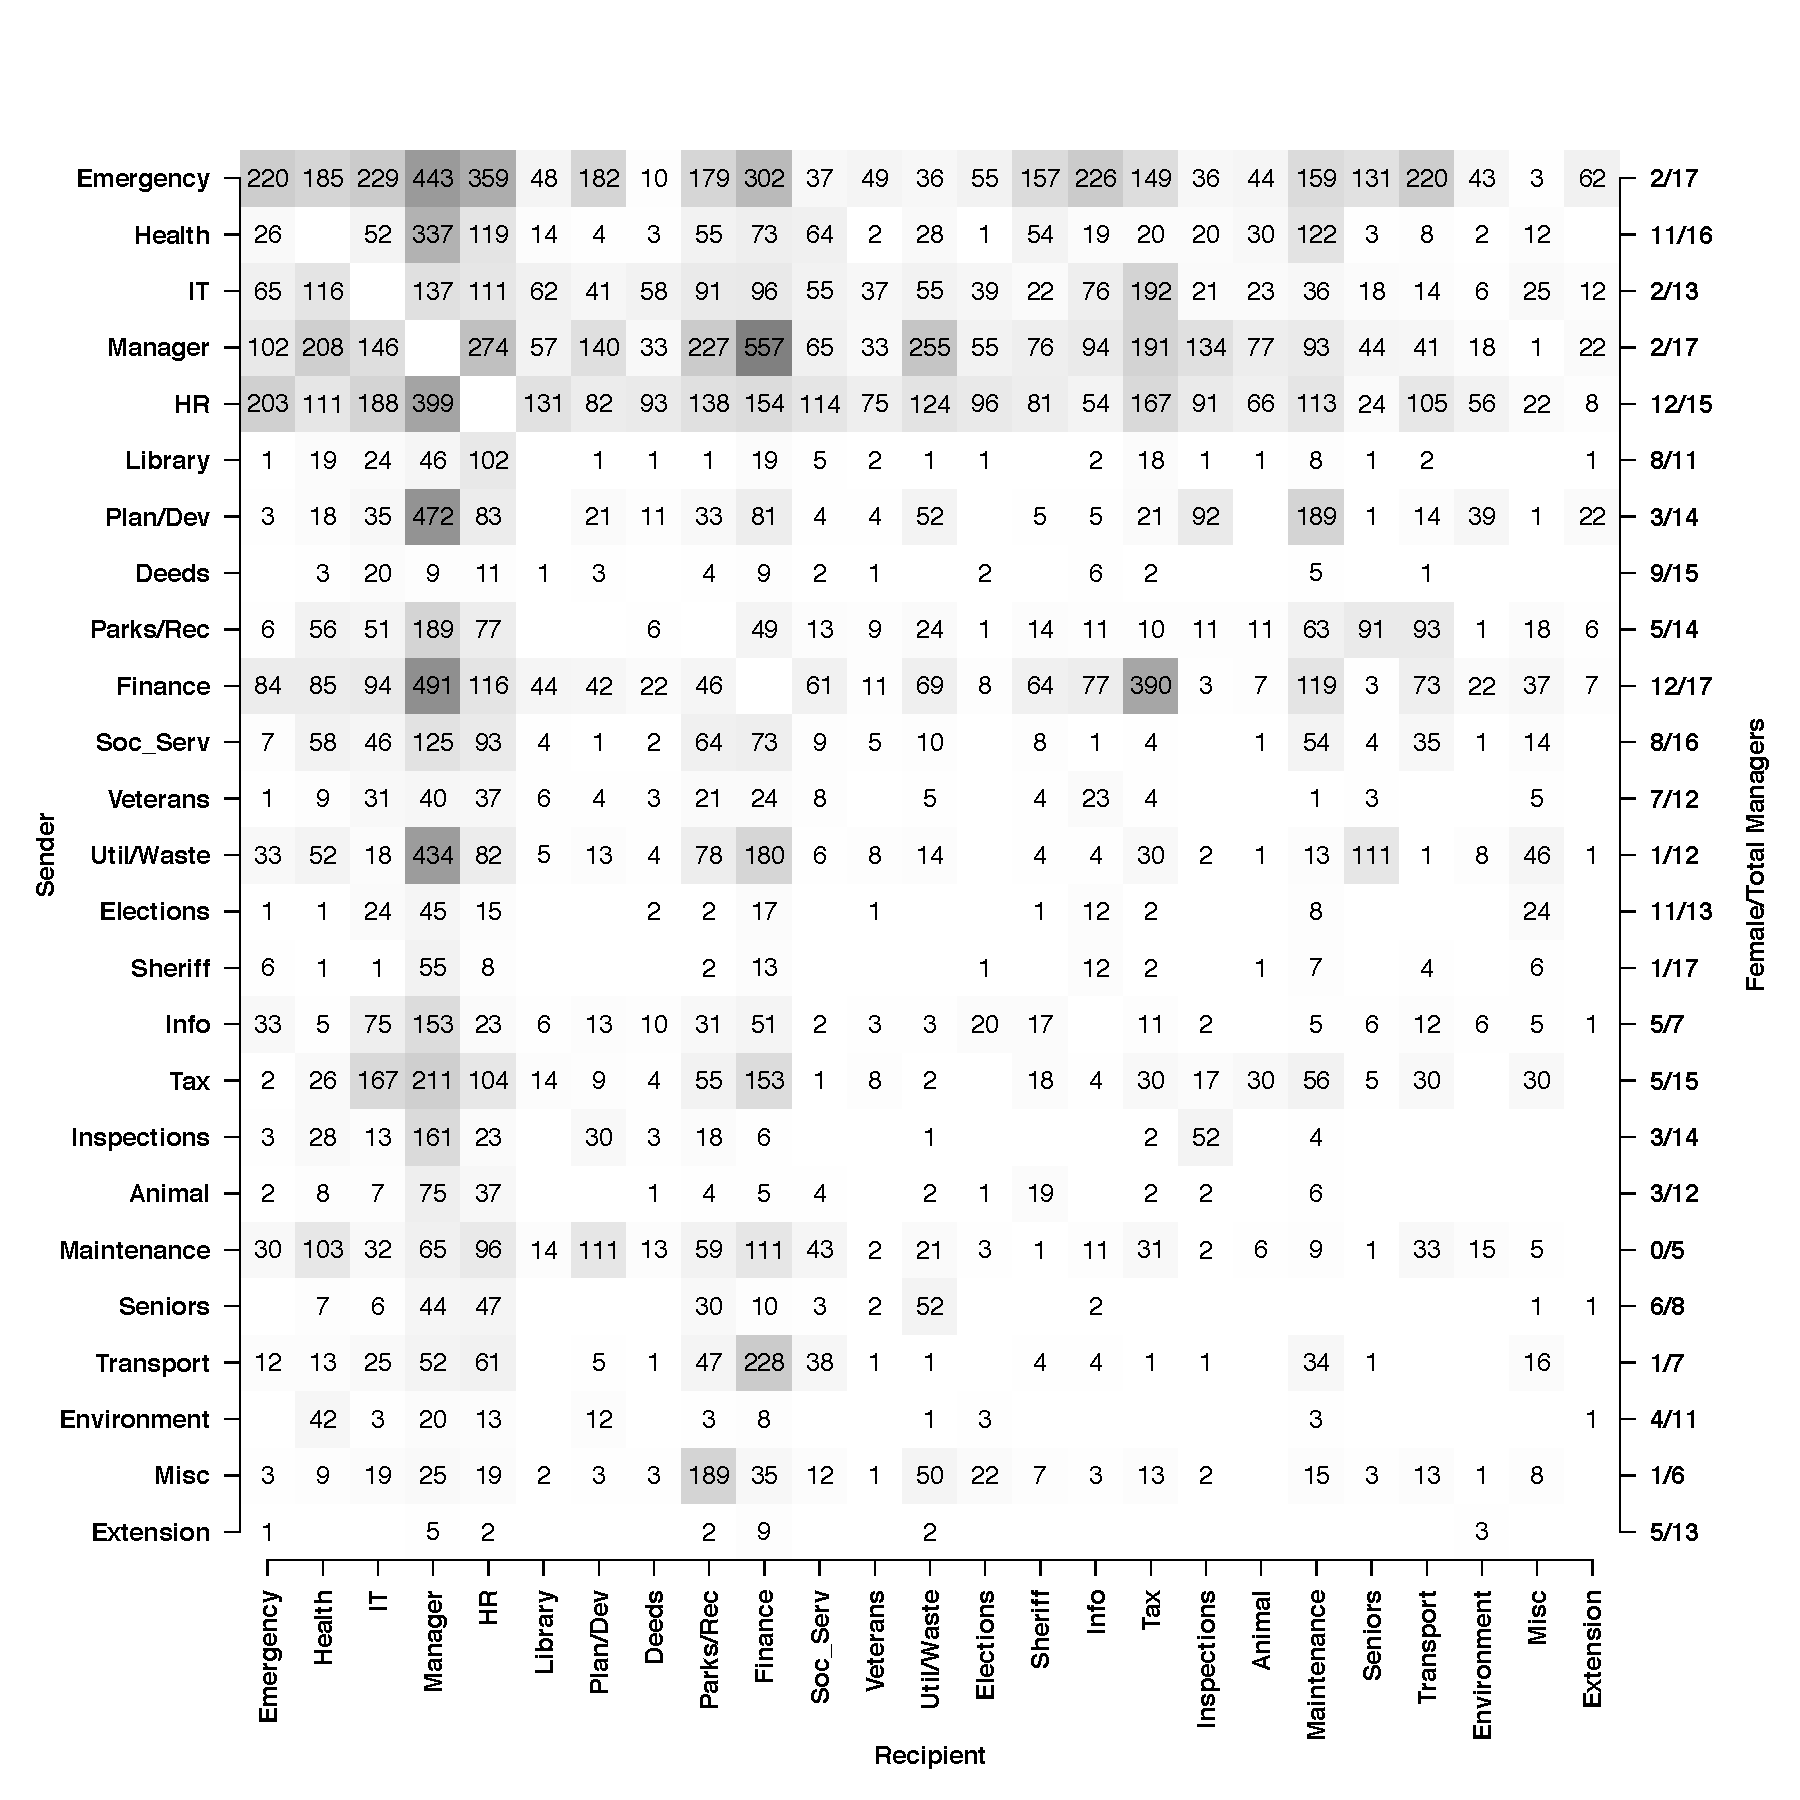
\includegraphics[width = 0.8\textwidth]{images/Aggregate_Email_Flows.pdf}
	\caption{\label{fig:heatmaps}Heat map depicting the number of emails sent from the row department to the column department aggregated across counties. Departments were also hand coded into one of 25 different categories based on given titles, to group departments that perform a similar function. The right margin displays the number of counties that had a manager of type X, and the number of those managers who were women.}
	\end{figure}
	% use recipeint rather than receiver and flip the y axis. omit zeros. have the shading march along together
	
	\item We can see that some departments are mostly men -- the county manager (the boss), the sheriff, and the emergency manager, for example. Others are mostly women -- the HR, finance, health, for example. 
	\item So there is some evidence of gendering in positions, but what about men and women who perform the same position? 
	
	\item What we want to know is whether the gender of an email sender and its recipients is independent of the their respective departments. 
	
	\item To test for independence, we construct a contingency table of department dyad types (eg. finance -- HR) against gender dyad types (eg. male - female). We then perform a $\chi^2$ test for independence between the rows and columns.
	
	\item The test statistic is $\chi^2 = 37,404$ with a simulated p-value\footnote{We use bootstrapped p values calculated using 50,000 resamples as they are more conservative.} $< 0.00002$, indicating that the gender of an email sender and its recipients is not independent of the their respective departments.
	
	\item This indicates that there is gender bias in communication when we disaggregate to the department dyad level, however, we are still stuck.
	
	\item This analysis does not allow us to disentangle the two potential sources of the pattern we find -- bias in the positions women hold within these organizations, and bias in the way that male and female managers communicate. 
	
	\item Furthermore, this analysis may be slicing our data too thin since not all counties have a department manager of every type, and any particular department dyad may only exchange a handful of emails. Moreover, the department attribute of each manager is likely caused by several factors other than the topics of communication that may relate to gender bias. 
	
	\item One solution to the problems raised above is to model the email content, as general topics such as balancing budgets are commonly represented across counties. Practically, this also allows us to focus on a smaller number of communication topics that are shared across counties.
	
	\item To do this, we might want to use a statistical topic model to categorize emails, then model  gender mixing using the LSM in each topic.
	
	\item However, the gender mixing parameters we infer using this approach would be confounded by selection effects. As a toy example, we would not be able to tell whether men prefer to talk to male coworkers over female coworkers about football, or women prefer not to talk about football at work, and so they do not participate in those conversations. 
	
	\item To disentangle these effects, we need a joint model for email topical content, and the structure of communication.
	
\end{enumerate}
	
	%Departments in which managers work may provide a useful proxy measure for "topics of communication", so its insightful to at least look at department-specific patterns. However, using an available proxy to measure a concept raises a number of problems (e.g., departments may not be comparable across counties, we may be slicing our data too thin since there is only 1 or 2 representatives of each department in each county, general topics such as balancing budgets are commonly represented across counties, the department attribute of each manager is caused by several factors other than the topics of communication that may relate to gender bias). The justification for using our model is that the latent variables we infer reflect topic domains that are relevant in differentiating patterns of social interaction. The only data informing the variables we infer are the content of communication and the patterns of interaction. And by tuning the number of topics and social spaces we infer, we can control how thinly we divide our data, which is not possible to do with the department proxy. Instead of using a proxy out of convenience, we're doing the best we possibly can to operationalize our concepts using our data.
	
	% \item Lets look at an example of finance managers because every county has one. First off, there are only two female county managers and the finance managers in their counties are both women, so we focus instead on counties with male managers. Of these 15 counties, 10 have a female finance manager and 5 have a male finance manager. How do they communicate with the county manager?
%
%
% 	\begin{table}[H]
% 	\centering
% 		\begin{tabular}{m{2in}cc}
% 		\toprule
% 		& \multicolumn{2}{c}{Finance Mgr. Gender} \\
% 	& \textbf{Male} & \textbf{Female}  \\
% 		 \midrule
% 		 Emails Sent to County Manager & 48.4\%& 20.5\% \\
% 		  & (151/312) & (334/1628)\\
% 		 Percent of Emails Sent by County Manager to Finance Manager & 21.2\% & 24.2\% \\
% 		  & (182/859) & (372/1535)\\
% 		\bottomrule
% 		\end{tabular}
% 		\caption{\label{tab:finance stats}County manager -- finance manager communication for male county managers. Out of 15 counties with a male county manager, 10 had female finance managers and 5 had male finance managers. The (Fraction) displayed under each percentage is the raw number of emails sent to that manager divided by the total number of emails sent, aggregated over counties. }
% 	\end{table}
%
% 	\item Male county managers do not communicate preferentially with finance managers of either gender, so no evidence for biased treatment by supervisor within positions in this case.
% 	\item However, female finance managers are sending lots more emails on average (168) than their male counterparts (62), even though they send the same number to the county manager. Remember that on average, men and women send the same number of emails, so it is not just that women use email more in general. So are their job responsibilities different?
% 	\item To understand this, we need to look at email content -- what are male and female managers talking about?
% 	\item A quick and dirty way to start is by searching for things like question marks, exclamation points, and "Thanks" to see if we observe differences by gender.
	
	
	% # female finance managers send male county managers 20.5% (334/1628) of emails
	%   # male finance managers send male county managers 48.4% (151/312) of emails
	%   # male county managers send female finance managers 24.2% (372/1535) of emails
	%   # male county managers send male finance managers 21.2% (182/859) of emails
	
	
	% lets cut this
	% \begin{table}[H]
% 	\centering
% 	\begin{tabular}{m{2in}rrr}
% 	\toprule
% 	 \textbf{Email Content} & \textbf{Male} & \textbf{Female} & \textbf{t-test} \\
% 	 \midrule
% 	 Question Marks per Email Sent & 0.218 & 0.235 & 0.033\\
% 	 Exclamation Marks per Email Sent & 0.088 & 0.363 & 0.001\\
% 	 ``Thanks'' per Email Sent & 0.340 & 0.425 & 0.028 \\
% 	\bottomrule
% 	\end{tabular}
% 		\caption{\label{tab:Gender Aggregate Stats} Manager-to-manager email communication statistics by gender across all departments and all counties. The \textbf{t-test} column reports reports Welch 2-sample t-test $p$ values for difference in means where applicable. When calculating content statistics, only the body text was used so as to avoid double counting subject lines in responses.}
% 	\end{table}
%
% 	\item We do see significant differences, but why? Is this because men and women use language differently to accomplish the same goals, or because gender plays a role in the tasks managers are asked to do?
	


\section{A Model of Email Content}
\begin{enumerate}
	\item Motivation for building a model for email data -- who you send an email to depends on what it is about. And what you say depends on who you are talking to. 
	\item Our solution: a generative model for email topics and recipients. Then discuss the existing TPME model and why we build on it. 
	\item Overview of the generative process in plain english.
	\item Describe the generative process for LDA part of model.
	\item Model based topic clustering.
	\item Explain how draws of message recipients are conditioned on the email topics. 
	\item Describe the generative process for the latent space portion of model.
	\item Summarize the generative process and lead into inference. 
\end{enumerate}

\subsection{Inference}
\begin{enumerate}
	\item We have to invert the generative process to perform inference on the model parameters.
	\item We use block Metropolis Hastings within Gibbs sampling.
	\item A beta R package is available for those interested.
	\item Discuss our model specification and justify our hyper-parameter choices.
\end{enumerate}

\section{Gender Mixing}

\begin{enumerate}
	\item Since we have modeled content and structure together, we have broken up the confounding we were concerned about, and we can now interpret the gender mixing parameters that come out of our model with more confidence.
	
	\item Lets return to the question we posed at the end of our descriptive analysis section: is there gender bias in the patterns of communication in these county governments. 
	
	\item Add in Bruce's MV KS test results for each county here.
	
	\item Interpret the results.
	
	\item Take as a case study, a county with the highest degree of gender bias, as identified by this method.
	
	\item interpret the topic model output from two different clusters and discuss.
	
% 	\item  Lets form some expectations about the relationship between gender mixing parameters we estimate.
%
% 	\item If we observe a positive relationship between the female-female mixing parameters and the male-female or female-male mixing parameters we estimate, this is evidence that there are male and female topics, and if you want to talk about a female (male) topic, you send an email to a female (male) colleague. This is evidence for the gendering of communication content. As a toy example, if you want to email about football, you email a male colleague.
%
% 	\item If we observe a negative relationship, this is evidence that there are some things that men send or receive emails about, and some things women send or receive emails about. This is evidence for gender bias in organizational roles.
%
% 	\begin{figure}[H]
% 		\begin{tabular}{ccc}
% 			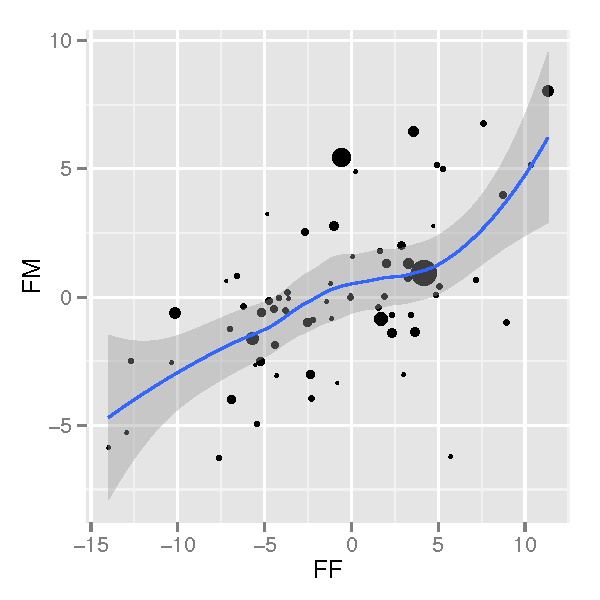
\includegraphics[width = 0.28\textwidth]{images/FF_FM.pdf} &
% 			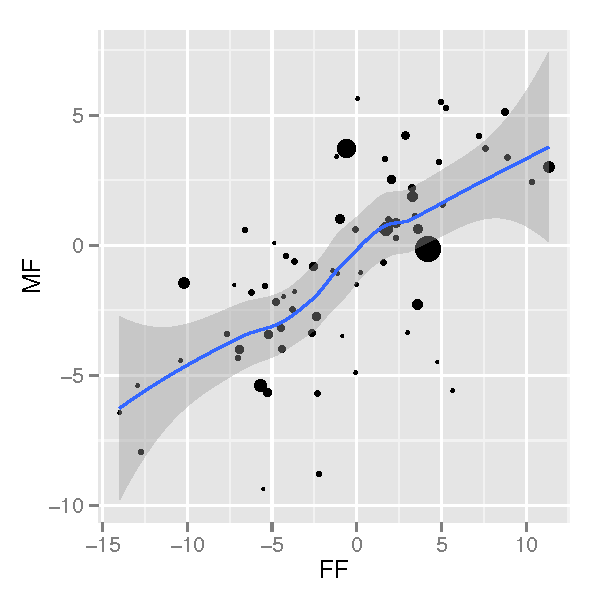
\includegraphics[width = 0.28\textwidth]{images/FF_MF.pdf}&
% 			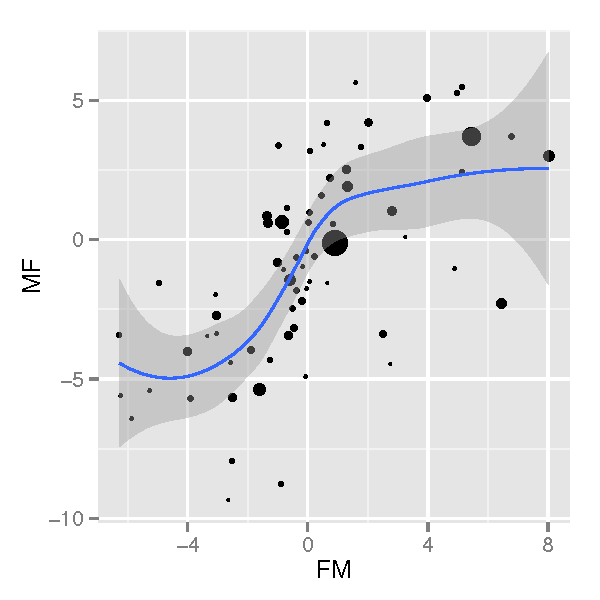
\includegraphics[width = 0.28\textwidth]{images/FM_MF.pdf}
% 		\end{tabular}
% 	\end{figure}
%
% \item We observe a pattern that is consistent with a gendering of communication content.
	
	
\end{enumerate}



% \begin{enumerate}
% 	\item Here, we test whether larger organizations exhibit less gender bias, which is something that \cite{Huffman2010} found using longitudinal data from the Employment Opportunity Commission on occupational status and pay.
% 	\item The key benefit of using our model in this context: we remove the confounding effect of what is being talked about on the relationship between gender mixing and organization size. For example, it could be that in aggregate, differences in gender mixing across counties are only be related to differences in how those organizations use email. Some might use email for more informal communication (\citep{Ibarra1992} found that informal communication is more homophilous) while others use it for more formal communication, leading to a difference in gender mixing that is unrelated to organization size.
% 	\item Display plots.
% 	\item Discuss our results, which indicate that cross-gender communication is most likely in mid-sized organizations.
% \end{enumerate}




\bibliography{PINLab}
\bibliographystyle{chicago}

\end{document}